\documentclass[a4paper]{article}
\usepackage[utf8]{inputenc}
\usepackage{fancyhdr}
\usepackage[margin=2.5cm]{geometry}
\usepackage{amsmath, amssymb}
\usepackage{aligned-overset}
\usepackage{graphicx}
\usepackage{float}


% eigene commands
\newcommand{\epszero}{\epsilon_0}
% partielle ableitungen in Kugelkoordinaten
\newcommand{\delr}{\partial_r}
\newcommand{\delp}{\partial_\phi}
\newcommand{\delt}{\partial_\theta}
% einheisvektoren in kugelkoordinaten
\newcommand{\er}{\hat{e}_r}
\newcommand{\et}{\hat{e}_\theta}
\newcommand{\ep}{\hat{e}_\phi}
% 1/4piepsilon0
\newcommand{\kco}{\frac{1}{4\pi\epsilon_0}}

\fancyhf{}
% vspaces in den headern fuer Distanzen notwendig
% linke Seite: Namen der Abgabegruppe
\lhead{\textbf{Etem Kalyon\\Matthias Maile\\Roman Surma}\vspace{1.5cm}}
% rechte Seite: Modul, Gruppe, Semester
\rhead{\textbf{Physik II - Gruppe 2\\Sommersemester 2020}\vspace{1.5cm}}
% Center: nr. des blattes
\chead{\vspace{2.5cm}\huge{\textbf{2. Übungsblatt}}}
% benoetigt damit der eigentliche Text nicht in der Überschrift steckt
\setlength{\headheight}{4cm} 


\begin{document}
% pagestyle nicht global festgelegt, da sonst bei allen Seiten Überschrift ist
% daher muss hier fancy aktiviert werden (für eine Seite, daher thispagestyle)
\thispagestyle{fancy}

\section*{Aufgabe 1}

\newpage
\setlength{\headheight}{0cm}

\section*{Aufgabe 2}
\paragraph{a)}
Der Laplace-Operator $\Delta$ in Kugelkoordinaten:
\[
	\Delta =
	\frac{1}{r} \partial_r^2r 
	+ \frac1{r^2\sin\theta} \partial_\theta
	\left(
		\sin\theta \partial_\theta
	\right)
	+
	\frac1{\sin^2\theta} \partial_\varphi^2
\]
Aus der Ladungsverteilung $\rho$ und der Poisson-Gleichung folgen:
\[
	\Delta \phi = 
	\begin{cases}
		-\frac{\rho_0}{\epszero} &\text{für } r \leq R \\
		0 &\text{für } r > R
	\end{cases}
\]
Die Ladungsverteilung besitzt eine Kugelsymmetrie, daher wird es sich auch
bei dem Potential um eine größe handeln, die lediglich von der Distanz $r$
abhängen wird.\\
Die partiellen Ableitung $\partial_\varphi\phi$ und $\partial_\theta\phi$ 
sind daher 0 und können vernachlässigt werden.\\
Für $r > R$ folgt dann:
\begin{align*}
	\Delta \phi
	= \frac1r \partial_r^2 \left(r * \phi) \right)
	&= \rho(r > R) = 0\\
	% r auf andere seite
	\Leftrightarrow
	\partial_r^2 \left(r * \phi) \right) 
	&= 0 \\
	% 1. integrieren
	\Leftrightarrow
	\partial_r \left(r * \phi) \right) 
	&= \alpha \\
	% 2. integrieren
	\Leftrightarrow
	r * \phi
	&= \alpha * r + \beta \\
	% durch r kuerzen
	\Leftrightarrow
	\phi
	&= \alpha + \frac\beta r 
\end{align*}
$r \leq R$ folgt analog:
\begin{align*}
	\Delta \phi
	= \frac1r \partial_r^2 \left(r * \phi) \right)
	&= -\frac{\rho_0}{\epszero} \\
	% r auf andere seite
	\Leftrightarrow
	\partial_r^2 \left(r * \phi) \right) 
	&= -\frac{r * \rho_0}{\epszero} \\
	% 1. integrieren
	\Leftrightarrow
	\partial_r \left(r * \phi) \right)
	&= -\frac{\rho_0}{2 * \epszero} r^2 + \gamma \\
	% 2. integrieren
	\Leftrightarrow
	r * \phi
	&= -\frac{\rho_0}{6 * \epszero} r^3 + \gamma * r + \delta \\
	% durch r teilen
	\Leftrightarrow
	\phi
	&= -\frac{\rho_0}{6 * \epszero} r^2 + \gamma + \frac\delta r 
\end{align*}
Somit lautet das Potential $\phi$:
\[
	\phi(r) =
	\begin{cases}
		-\frac{\rho_0}{6 * \epszero} r^2 + \gamma + \frac\delta r
		&\text{für } r \leq R \\
		\alpha + \frac\beta r 
		&\text{für } r > R
	\end{cases}
\]

\newpage
\paragraph{b)}
Für ein eindeutiges Potential benötigen wir (da wir 4 Konstanten $\alpha, \beta, \gamma, \delta$ in der Gleichung haben) 4 Randbedingen:
\begin{enumerate}
	% endlich fuer r rightarrow 0
	\item $\phi$ endlich für $r\rightarrow 0$, damit wir ein für $r=0$ 
		ein eindeutiges Potential bestimmen können:
		\[
			\phi(0) = \lim_{r\rightarrow0} 
			-\frac{\rho_0}{6 * \epszero} r^2 
			+ \gamma 
			+ \frac\delta r
			= \lim_{r\rightarrow0} + \gamma
			+ \frac\delta r \overset{!}{\neq} \infty
			\Rightarrow
			\delta = 0
		\]
	% 0 fuer r = infty
	\item $\lim_{r\rightarrow\infty} \phi(r) = 0$ ist eine sinnvolle 
		Annahme, weil dadurch der ``Referenzpunkt`` des Potentials 
		$\infty$ ist. Für $\phi$ folgt dann:
		\[
			\lim_{r\rightarrow\infty}
			\phi(r) 
			= \lim_{r\rightarrow\infty}
			\alpha + \frac\beta r 
			= \alpha 
			\overset{!}{=} 0
			\Rightarrow
			\alpha = 0
			\]
	% stetigkeit bei r = R
	\item Stetigkeit des Potentials bei $r = R$ ist notwendig, um keine
		Sprungstellen zu erhalten.
		\[
			\limsup_{r\rightarrow R} \phi(r)
			\overset{!}{=}
			\liminf_{r\rightarrow R} \phi(r)
			\Rightarrow
			\frac{\beta}{R} = 
			\frac{-\rho_0 R^2}{6 \epszero} + \gamma
			\Rightarrow
			\gamma = 
			\frac\beta R + \frac{\rho_0}{6 \epszero} R^2
		\]
	\item Stetigkeit der ersten Ableitung des Potentials:
		\[
			\phi^\prime(r) = 
			\begin{cases}
				-\frac{\beta}{r^2}
				&\text{für } r > R \\
				-\frac{\rho}{3\epszero} r
				&\text{für } r \leq R
			\end{cases}
		\]
		\[
			\limsup_{r\rightarrow R} \phi^\prime(r)
			\overset{!}{=}
			\liminf_{r\rightarrow R} \phi^\prime(r)
			\Rightarrow
			\frac{-\beta}{R^2} =
			\frac{-\rho_0 R}{3 \epszero}
			\Rightarrow
			\beta
			=
			\frac{\rho_0 R^3}{3 \epszero}
		\]
\end{enumerate}
Wenn man den Wert für $\beta$ aus 4. in bei $\gamma$ einsetzt, erhalten wir
unser eindeutiges Potential:
\[
	\gamma = \frac\beta R + \frac{\rho_0}{6 \epszero} R^2
	=
	\frac{\rho_0 R^2}{3 \epszero} + 
	\frac{\rho_0 R^2}{6 \epszero}
	= 
	R^2 \frac{\rho_0}{2 \epszero}
\]
\paragraph{c)}
\mbox{}
\begin{figure}[H]
	\centering
	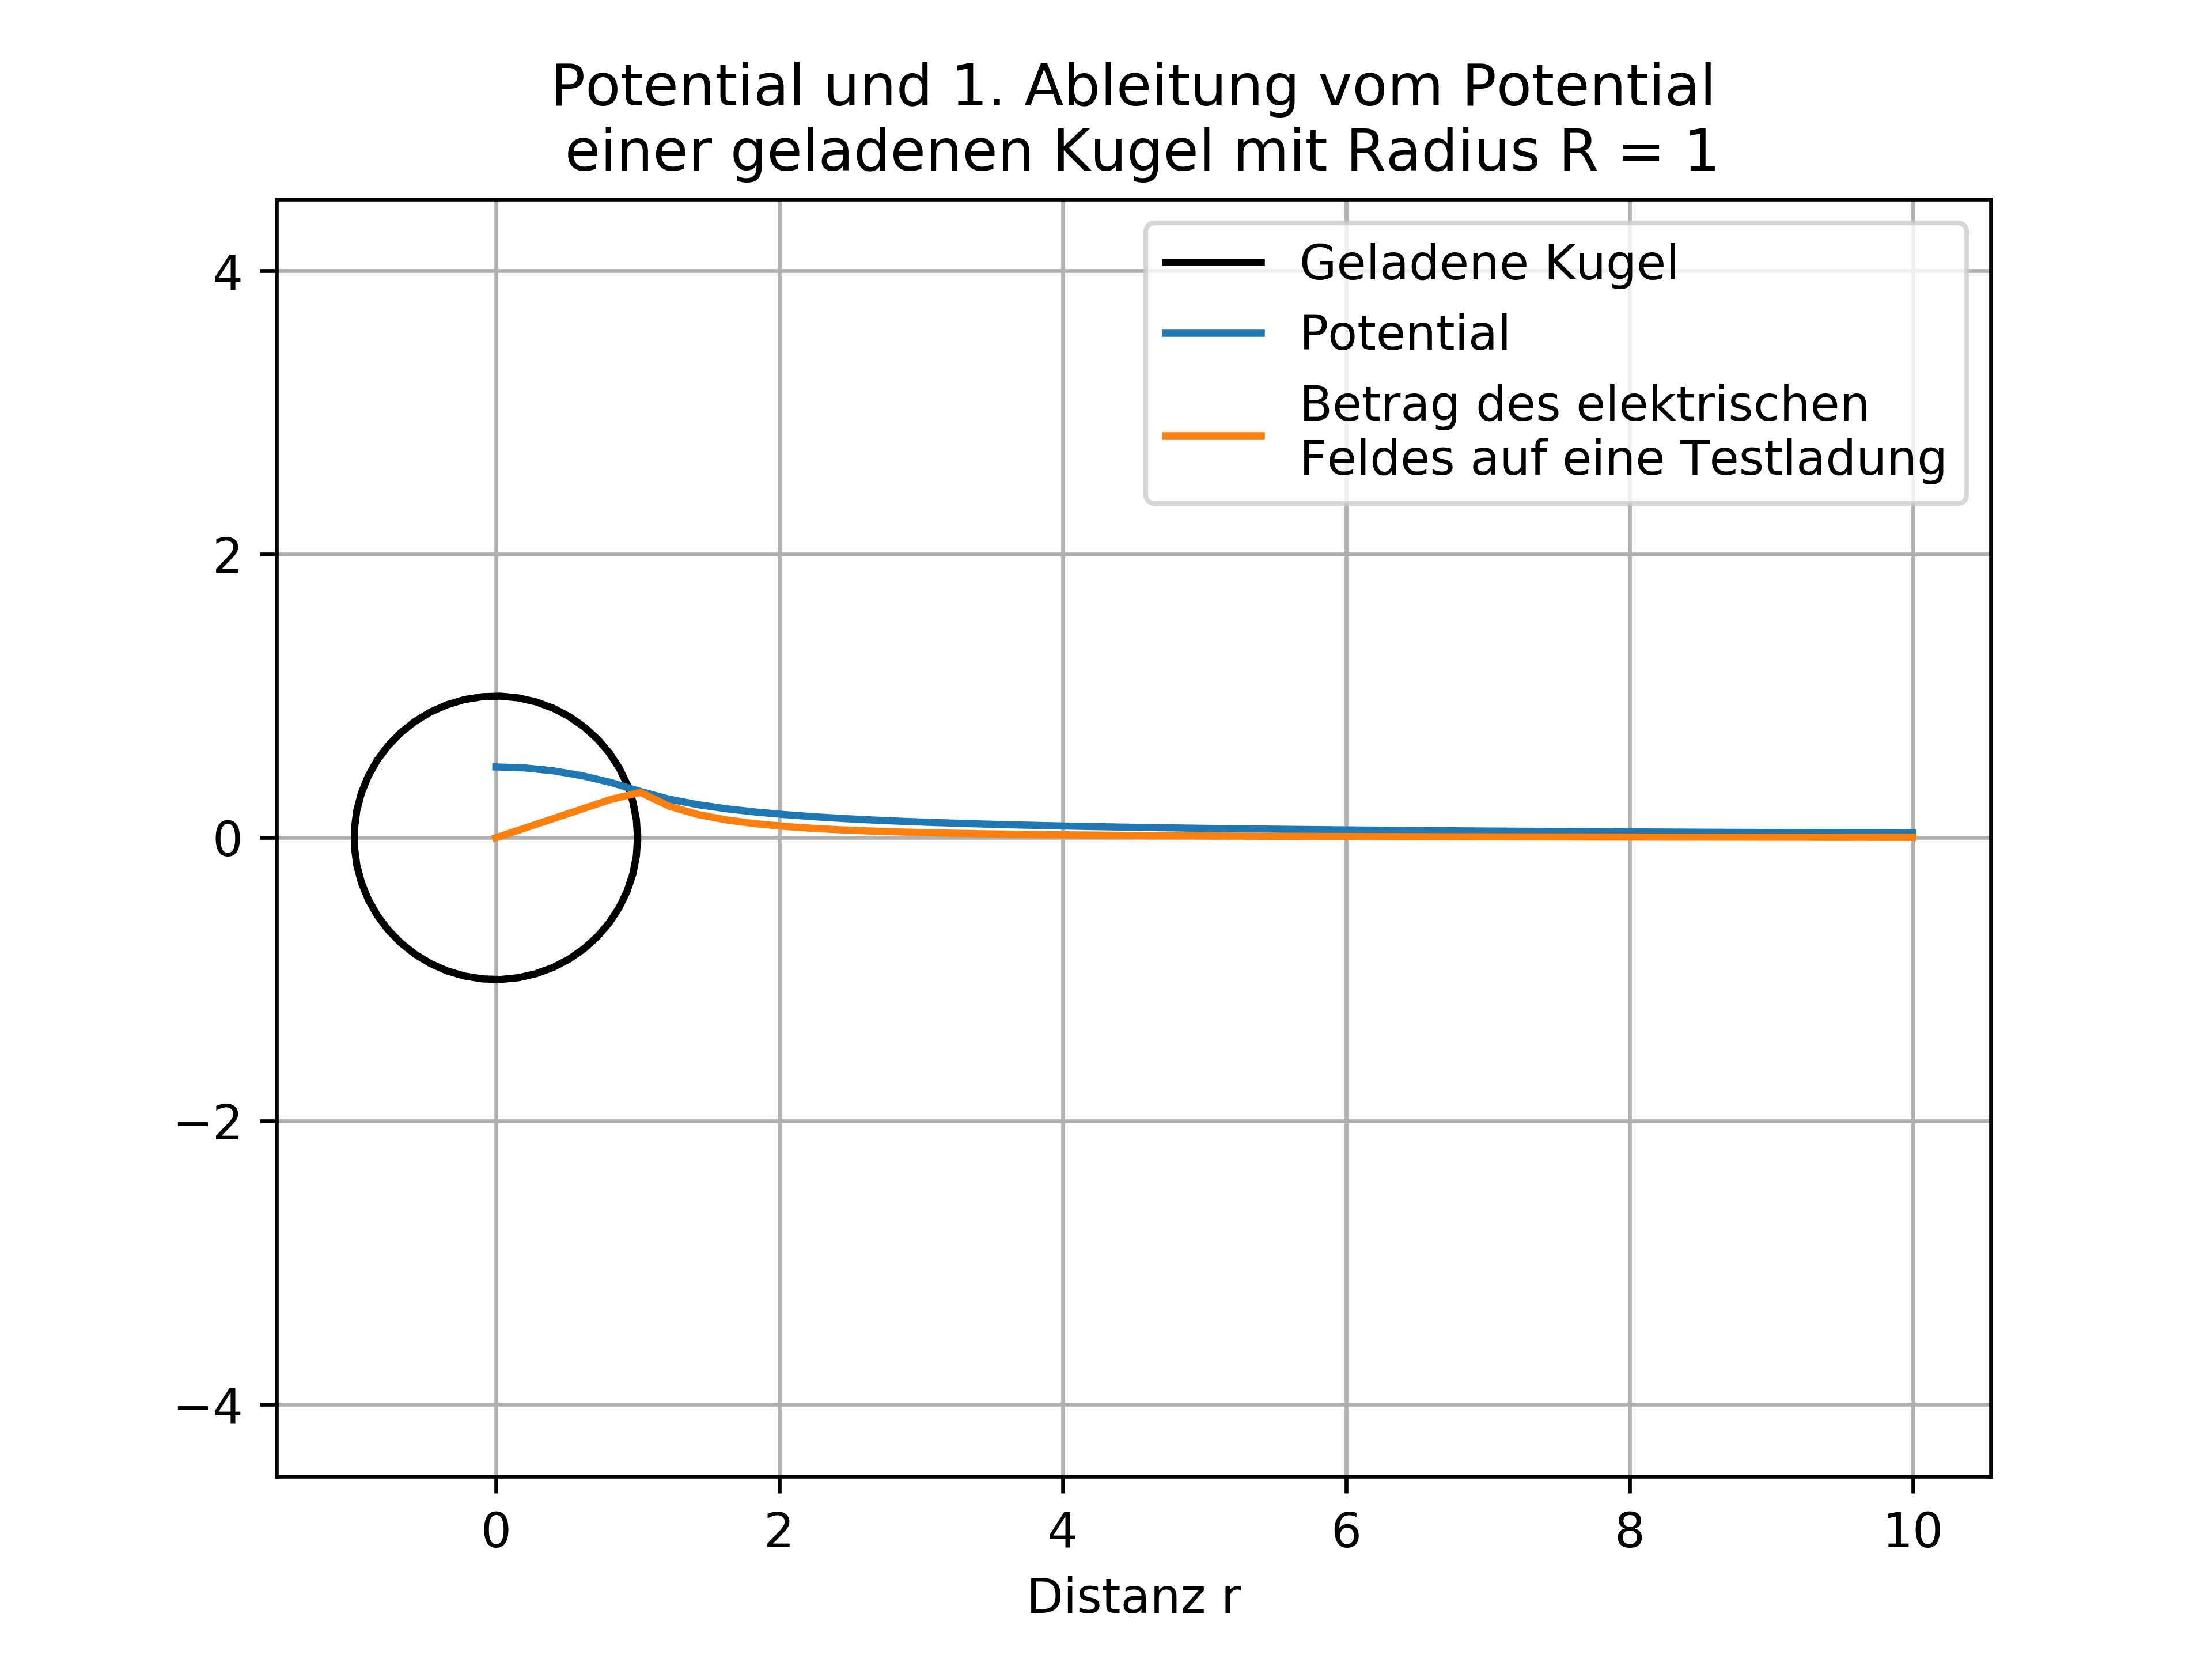
\includegraphics[width=15cm]{aufgabe2_efeld_analytisch.png}
\end{figure}
\newpage

\section*{Aufgabe 3}
\section*{Aufgabe 4}
\section*{Aufgabe 5}

\end{document}
